\section{Werkpakket 2: Prototyping}
2. Prototyping V0.1 (4 maanden) 

Het doel van het prototype is om zo snel mogelijk alle afzonderlijke stappen te testen en bewijzen dat het werkt. Het zal in een virtuele omgeving draaien waarbij makkelijk geïtereerd kan worden. Portabolt zal een interface ontwikkelen waarmee extern de batterijen aangestuurd kunnen worden. Er zal een communicatielaag worden gebouwd waarmee AIP de batterijen kan aansturen. Er wordt een testprotocol ontwikkeld waarmee elke afzonderlijke stap getest en gevalideerd kan worden. 
Deliverables: 
1. Portabolt sturingsinterface 
2. Koppeling tussen All in power, Portabolt, Edge, Envitron 
3. Werkend prototype in gesimuleerde omgeving 

Uren begroot: 1720

Opbouwen van de sandbox. We gaan eerst alles in dit prototype volledig digitaal ontwikkelen om te kijken of het werkt en waar we tegen aan lopen. Daarvoor gaan we een aantal simulaties ontwikkelen. 

\usepackage{placeins}  % Voeg dit toe aan je preamble

\subsection{1. Price Generation Module}
\textbf{Objective:} Simuleer dynamische elektriciteitsprijzen die elke dag om 12:00 uur gegenereerd worden voor de volgende dag. \\
\textbf{Input:} Random variabelen die de prijzen beïnvloeden (bijv. vraag, aanbod, weersomstandigheden). \\
\textbf{Output:} Een array met 24 prijzen, één voor elk uur van de volgende dag.

\begin{figure}[h!]
  \centering
  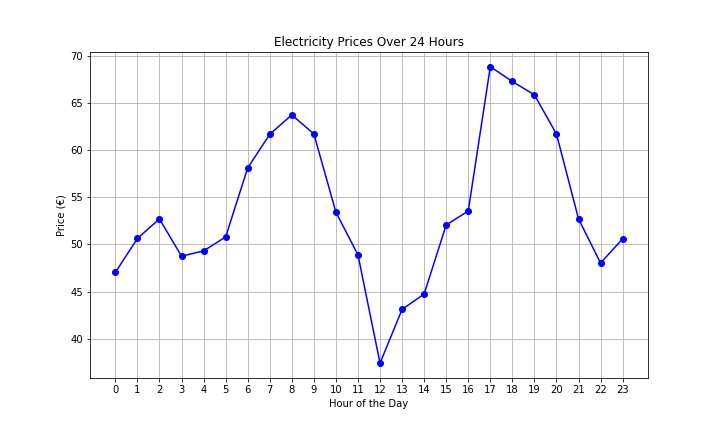
\includegraphics[width=\textwidth]{C:/GIT/Work/MIT AIP/docs/figures/price_generation_plot.png}
  \caption{Electricity Prices Over 24 Hours}
  \label{fig:price_plot}
\end{figure}

\FloatBarrier  % Voorkomt dat de afbeelding voorbij dit punt zweeft

\subsubsection{2. Energy Profile Simulation}
\textbf{Objective:} Creëer een energieverbruiksprofiel voor een gemiddeld bedrijf, dat per uur varieert. \\
\textbf{Input:} Kenmerken van het bedrijf (bijv. grootte, type industrie). \\
\textbf{Output:} Een array met 24 energieverbruikswaarden, één voor elk uur van de dag.

\subsubsection{3. Optimization Module (Trading Algorithm)}
\textbf{Objective:} Beslis wanneer elektriciteit moet worden gekocht of verkocht, gebaseerd op prijsfluctuaties en het energieverbruik van het bedrijf. \\
\textbf{Input:} Prijsarray en energieverbruiksarray. \\
\textbf{Output:} Een optimalisatiestrategie die maximale winst oplevert door elektriciteit op het laagste punt te kopen en op het hoogste punt te verkopen.
